% Poster, 48 x 36 in. Build from this folder: tectonic poster.tex   (figures: python poster/make_figures.py)
\documentclass{article}
\usepackage[paperwidth=48in,paperheight=36in,margin=0in]{geometry}
\usepackage{fontspec}
\setmainfont{texgyreheros}[Extension=.otf, UprightFont=*-regular, BoldFont=*-bold, ItalicFont=*-italic,
                           BoldItalicFont=*-bolditalic]
\usepackage{unicode-math}
\setmathfont{texgyredejavu-math.otf}
\usepackage{graphicx}
\usepackage{xcolor}
\usepackage{tikz}
\usetikzlibrary{arrows.meta,positioning,calc}
\usepackage{enumitem}
\pagestyle{empty}
\hyphenpenalty=10000
\exhyphenpenalty=10000
\setlength{\parindent}{0pt}
\setlength{\parskip}{0.45em}

\definecolor{blue}{HTML}{003262}
\definecolor{gold}{HTML}{C4820E}
\definecolor{ink}{HTML}{1A1A1A}
\definecolor{muted}{HTML}{555555}
\definecolor{tint}{HTML}{EEF2F8}

\newcommand{\body}{\fontsize{34}{45}\selectfont}
\newcommand{\note}{\fontsize{27}{35}\selectfont\color{muted}}
\newcommand{\heading}[1]{\vspace{1.1em}{\fontsize{52}{60}\selectfont\bfseries\color{blue}#1}\par\vspace{0.35em}}
\newcommand{\stat}[2]{{\fontsize{80}{84}\selectfont\bfseries\color{blue}#1}\\[0.2em]{\body #2}}

\begin{document}
\color{ink}
% ----- header -------------------------------------------------------------------------------------------------------
\begin{tikzpicture}[remember picture,overlay]
  \fill[blue] (current page.north west) rectangle ([yshift=-5.0in]current page.north east);
  \node[anchor=north west,text=white,align=left] at ([xshift=1.4in,yshift=-0.85in]current page.north west) {%
    {\fontsize{96}{108}\selectfont\bfseries Learning fixed-wing control at the actuator level}\\[0.35em]
    {\fontsize{96}{108}\selectfont\bfseries with the recipe of \emph{Learning to Fly in Seconds}}\\[0.6em]
    {\fontsize{44}{52}\selectfont Clément Dumeril \quad·\quad MEng capstone, Agile Robotics and Perception Lab,
     UC Berkeley \quad·\quad advisor: Giuseppe Loianno}};
  \node[anchor=north east,fill=white,rounded corners=10pt,inner sep=18pt] at ([xshift=-1.4in,yshift=-0.9in]current page.north east) {%
    
\includegraphics[height=1.55in]{logos/berkeley_engineering.png}\hspace{0.6in}%
    
\includegraphics[height=1.55in]{logos/arpl.png}};
\end{tikzpicture}

\vspace*{5.5in}
\hspace*{1.4in}%
% ----- column 1 -----------------------------------------------------------------------------------------------------
\begin{minipage}[t]{13.2in}
\body
\heading{Question}
Can a policy that moves an airplane's control surfaces and throttle directly, at 50~Hz and with no autopilot below,
be trained in minutes with the chain that flies quadrotors in \emph{Learning to Fly in Seconds}~[1] (its
simulator structure, update intervals and reward form, here with SAC), and follow a moving point to within a meter?

\heading{Three steps}
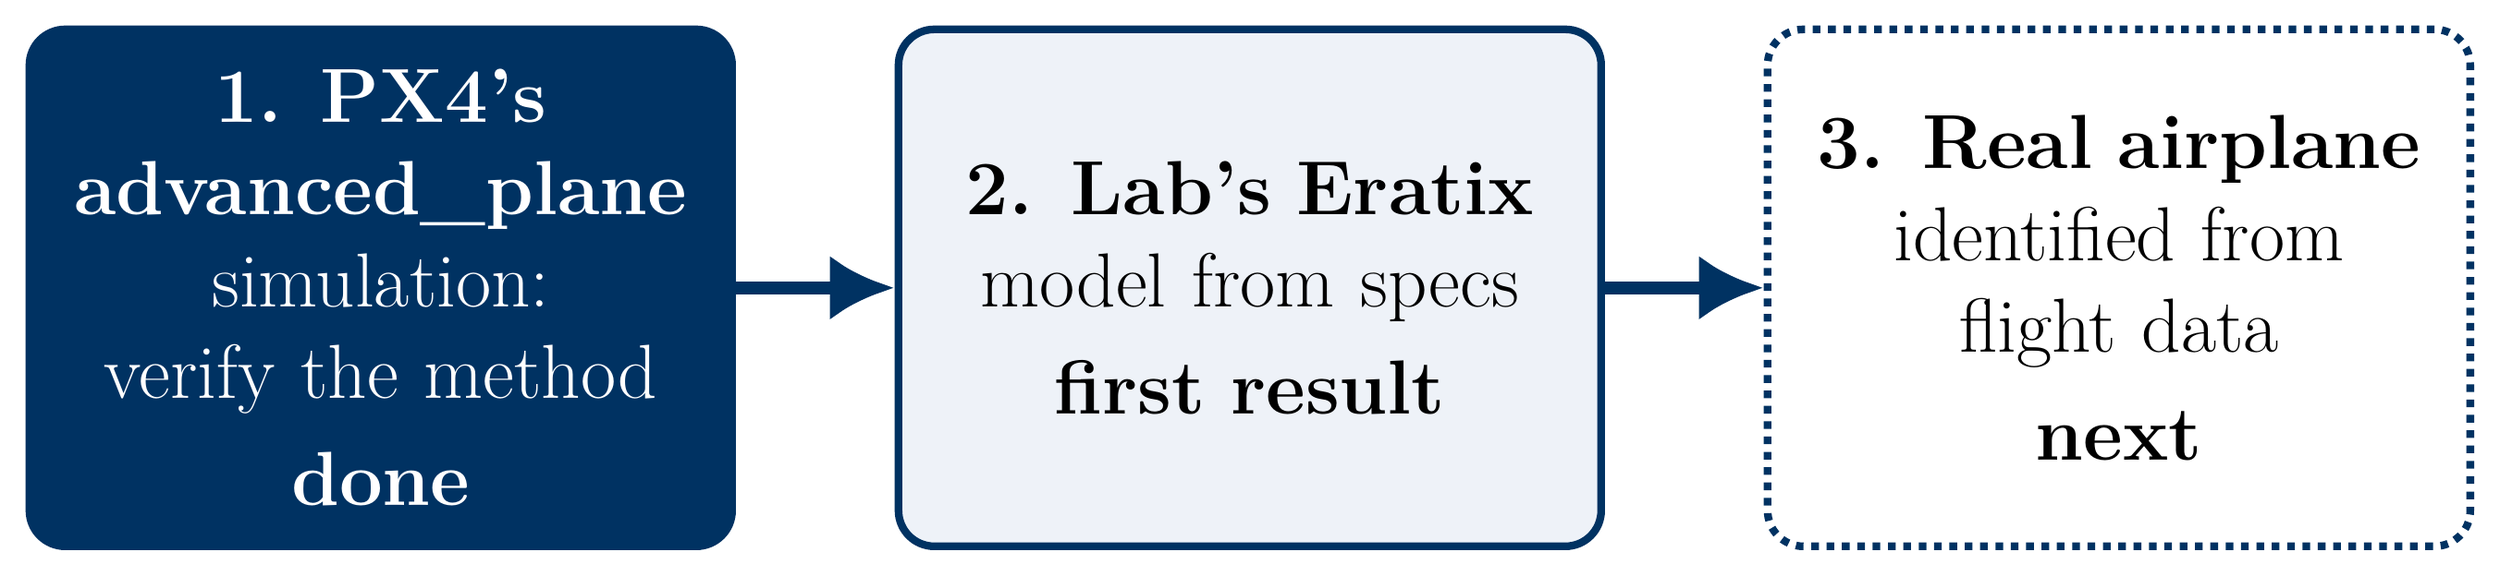
\begin{tikzpicture}[x=1in,y=1in,
    stage/.style={draw=blue,line width=3pt,rounded corners=14pt,minimum width=3.8in,text width=3.5in,minimum height=2.8in,align=center,
                 font=\fontsize{30}{36}\selectfont}]
  \node[stage,fill=blue,text=white] (a) at (0,0) {\textbf{1. PX4's}\\\textbf{advanced\_plane}\\simulation:\\verify the method\\[0.2em]\textbf{done}};
  \node[stage,fill=tint] (b) at (4.7,0) {\textbf{2. Lab's Eratix}\\model from specs\\[0.2em]\textbf{first result}};
  \node[stage,fill=white,dashed] (c) at (9.4,0) {\textbf{3. Real airplane}\\identified from\\flight data\\[0.2em]\textbf{next}};
  \draw[-{Latex[length=0.35in,width=0.35in]},line width=5pt,blue] (a) -- (b);
  \draw[-{Latex[length=0.35in,width=0.35in]},line width=5pt,blue] (b) -- (c);
\end{tikzpicture}

\heading{Method: the L2F chain}
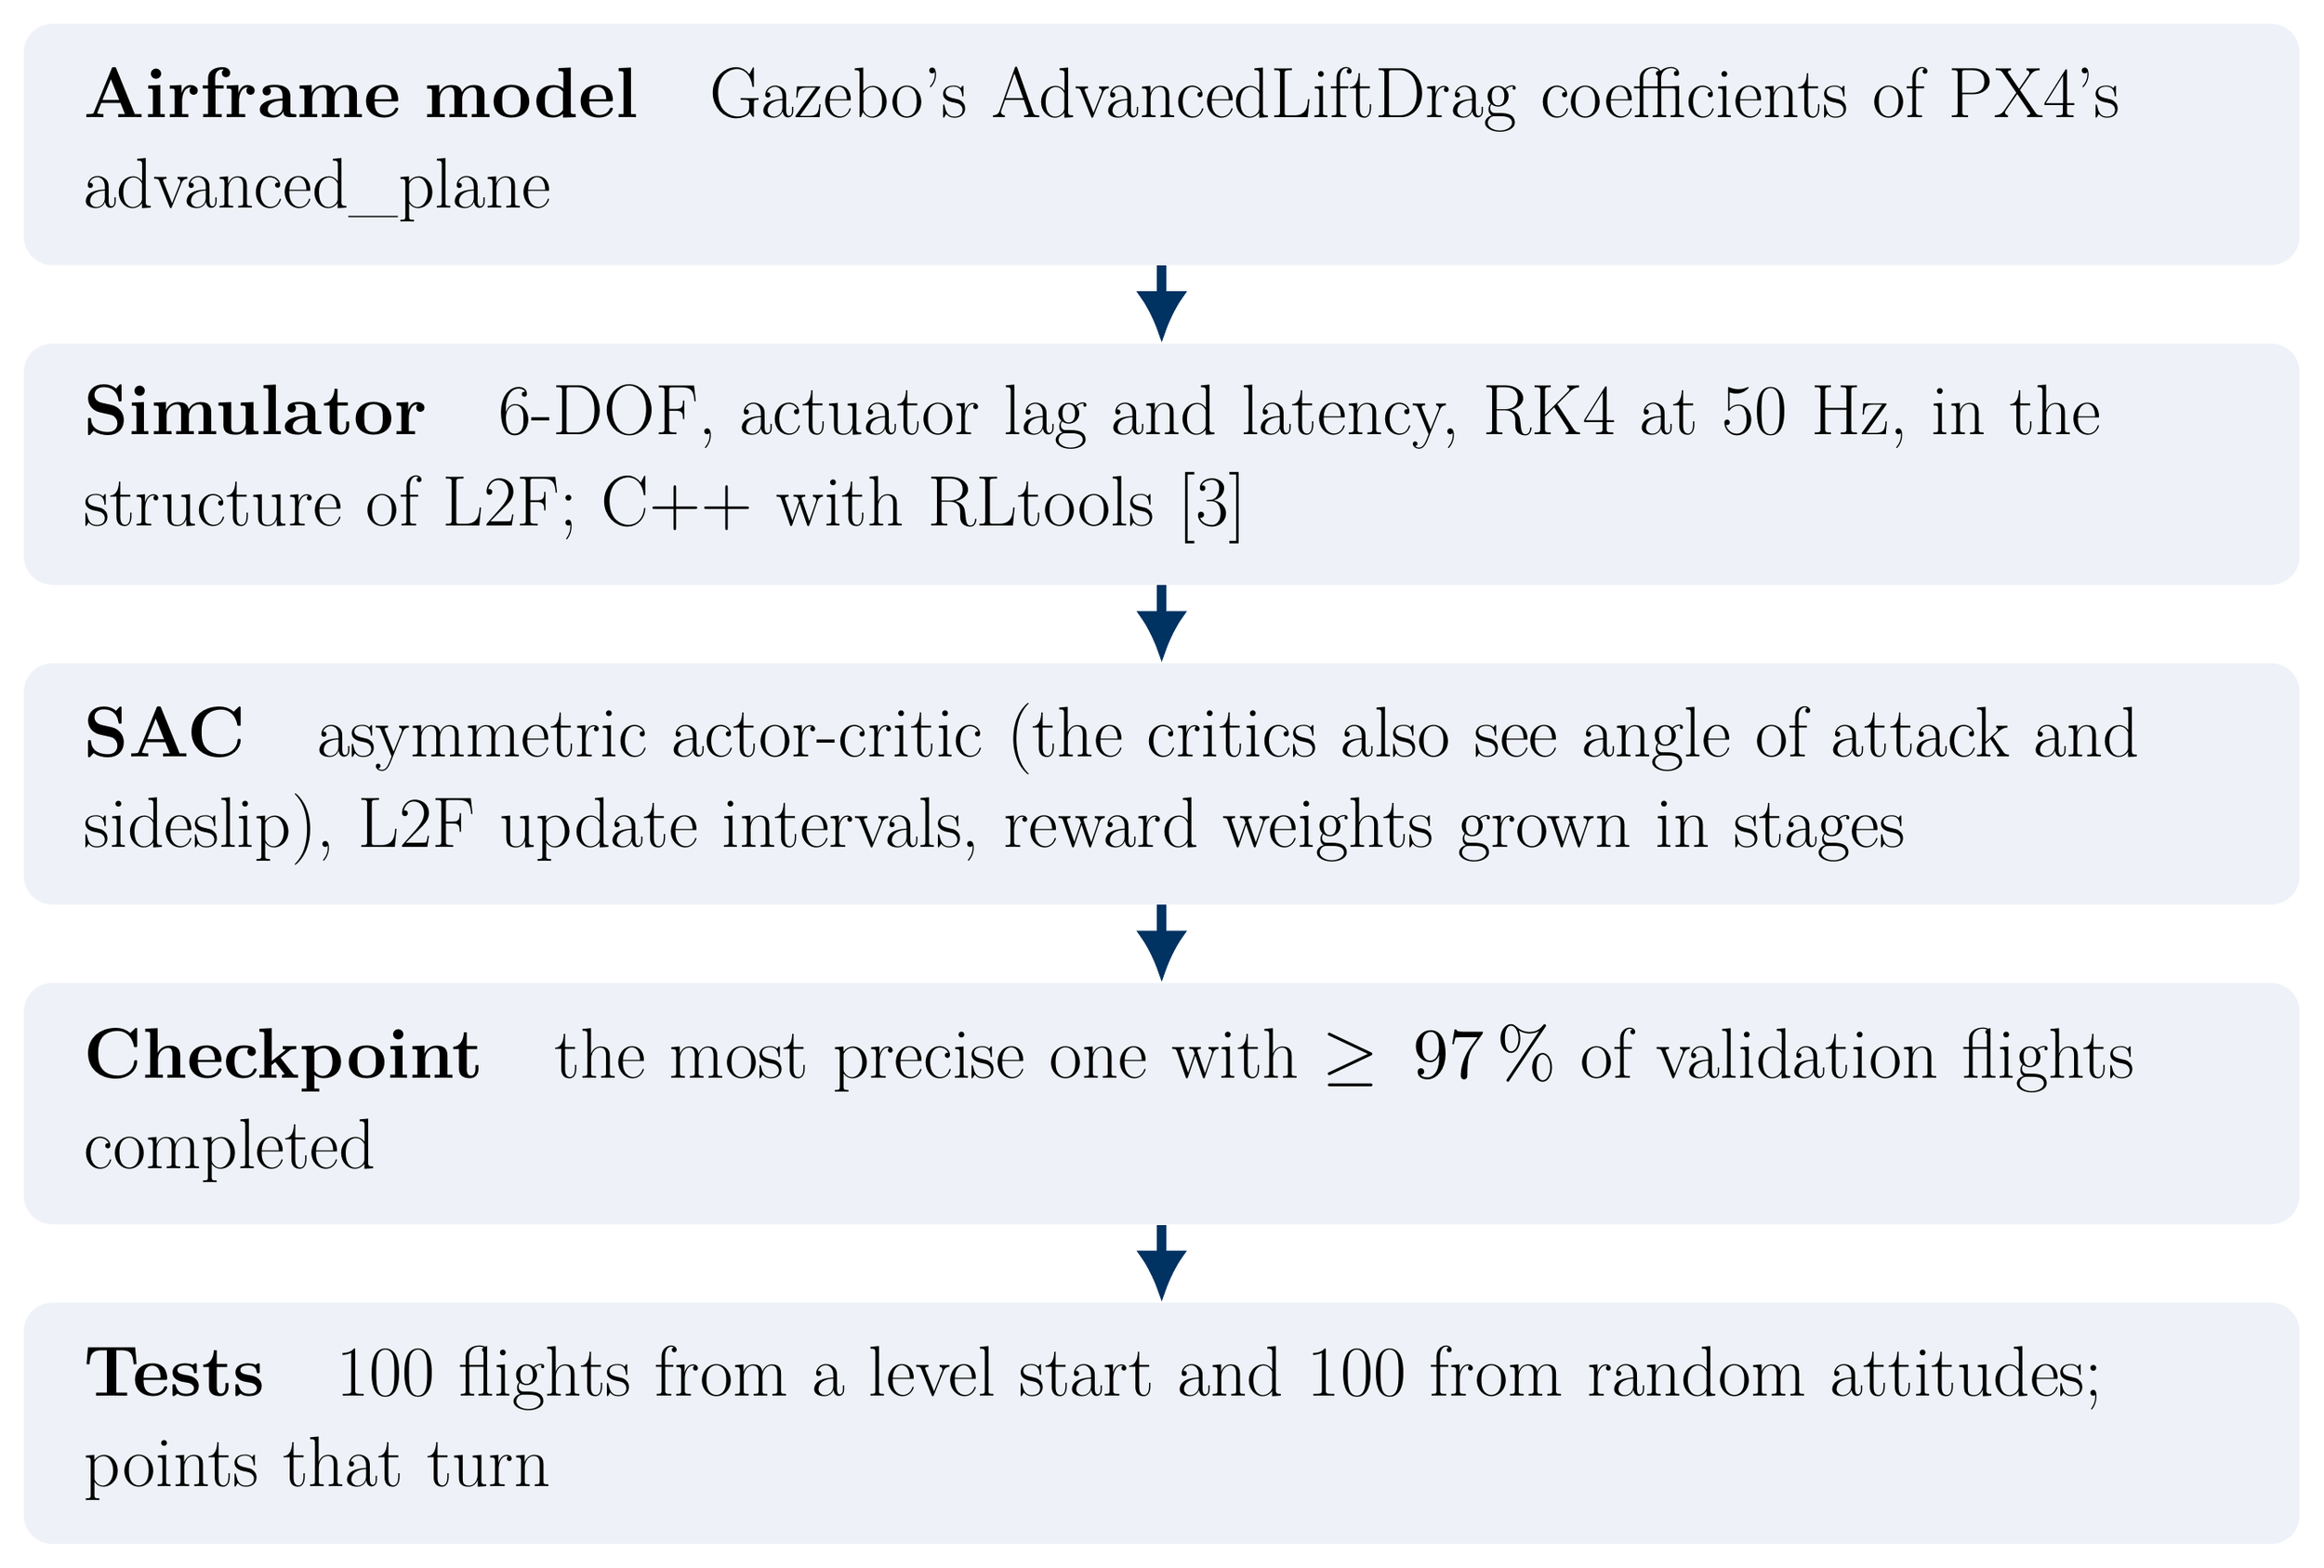
\begin{tikzpicture}[x=1in,y=1in,
    box/.style={fill=tint,rounded corners=12pt,minimum width=13.2in,minimum height=1.4in,align=left,text width=12.5in,
                font=\fontsize{30}{38}\selectfont},
    arr/.style={-{Latex[length=0.3in,width=0.3in]},line width=4pt,blue}]
  \node[box] (m) at (0,0) {\textbf{Airframe model}\quad Gazebo's AdvancedLiftDrag coefficients of PX4's advanced\_plane};
  \node[box,below=0.45in of m] (s) {\textbf{Simulator}\quad 6-DOF, actuator lag and latency, RK4 at 50~Hz, in the structure of L2F; C++ with RLtools~[3]};
  \node[box,below=0.45in of s] (t) {\textbf{SAC}\quad asymmetric actor-critic (the critics also see angle of attack and sideslip), L2F update intervals, reward weights grown in stages};
  \node[box,below=0.45in of t] (c) {\textbf{Checkpoint}\quad the most precise one with $\geq 97\,\%$ of validation flights completed};
  \node[box,below=0.45in of c] (e) {\textbf{Tests}\quad 100 flights from a level start and 100 from random attitudes; points that turn};
  \foreach \a/\b in {m/s,s/t,t/c,c/e} \draw[arr] (\a) -- (\b);
\end{tikzpicture}

{\note The C++ simulator matches the Python one to $7\times10^{-13}$ over 7,136 steps. An early policy flies the
airplane in PX4 SITL through ROS~2, where the simulator's one-step predictions have no bias against Gazebo
(accelerations within 0.2~m/s$^2$ and 0.2~rad/s$^2$).}

\heading{Task}
A point starts up to 50~m away and flies straight at 12--18~m/s; the airplane starts level, or in a random attitude
(bank $\pm60^\circ$, pitch $\pm20^\circ$), and must reach it and stay on it. Calm air, no sensor noise. The policy sees its position and velocity errors in the body frame
and its last commands.
\end{minipage}%
\hspace{1.0in}%
% ----- column 2 -----------------------------------------------------------------------------------------------------
\begin{minipage}[t]{16.8in}
\body
\heading{Step 1: precision, from 9.8~m to 1.4~m}
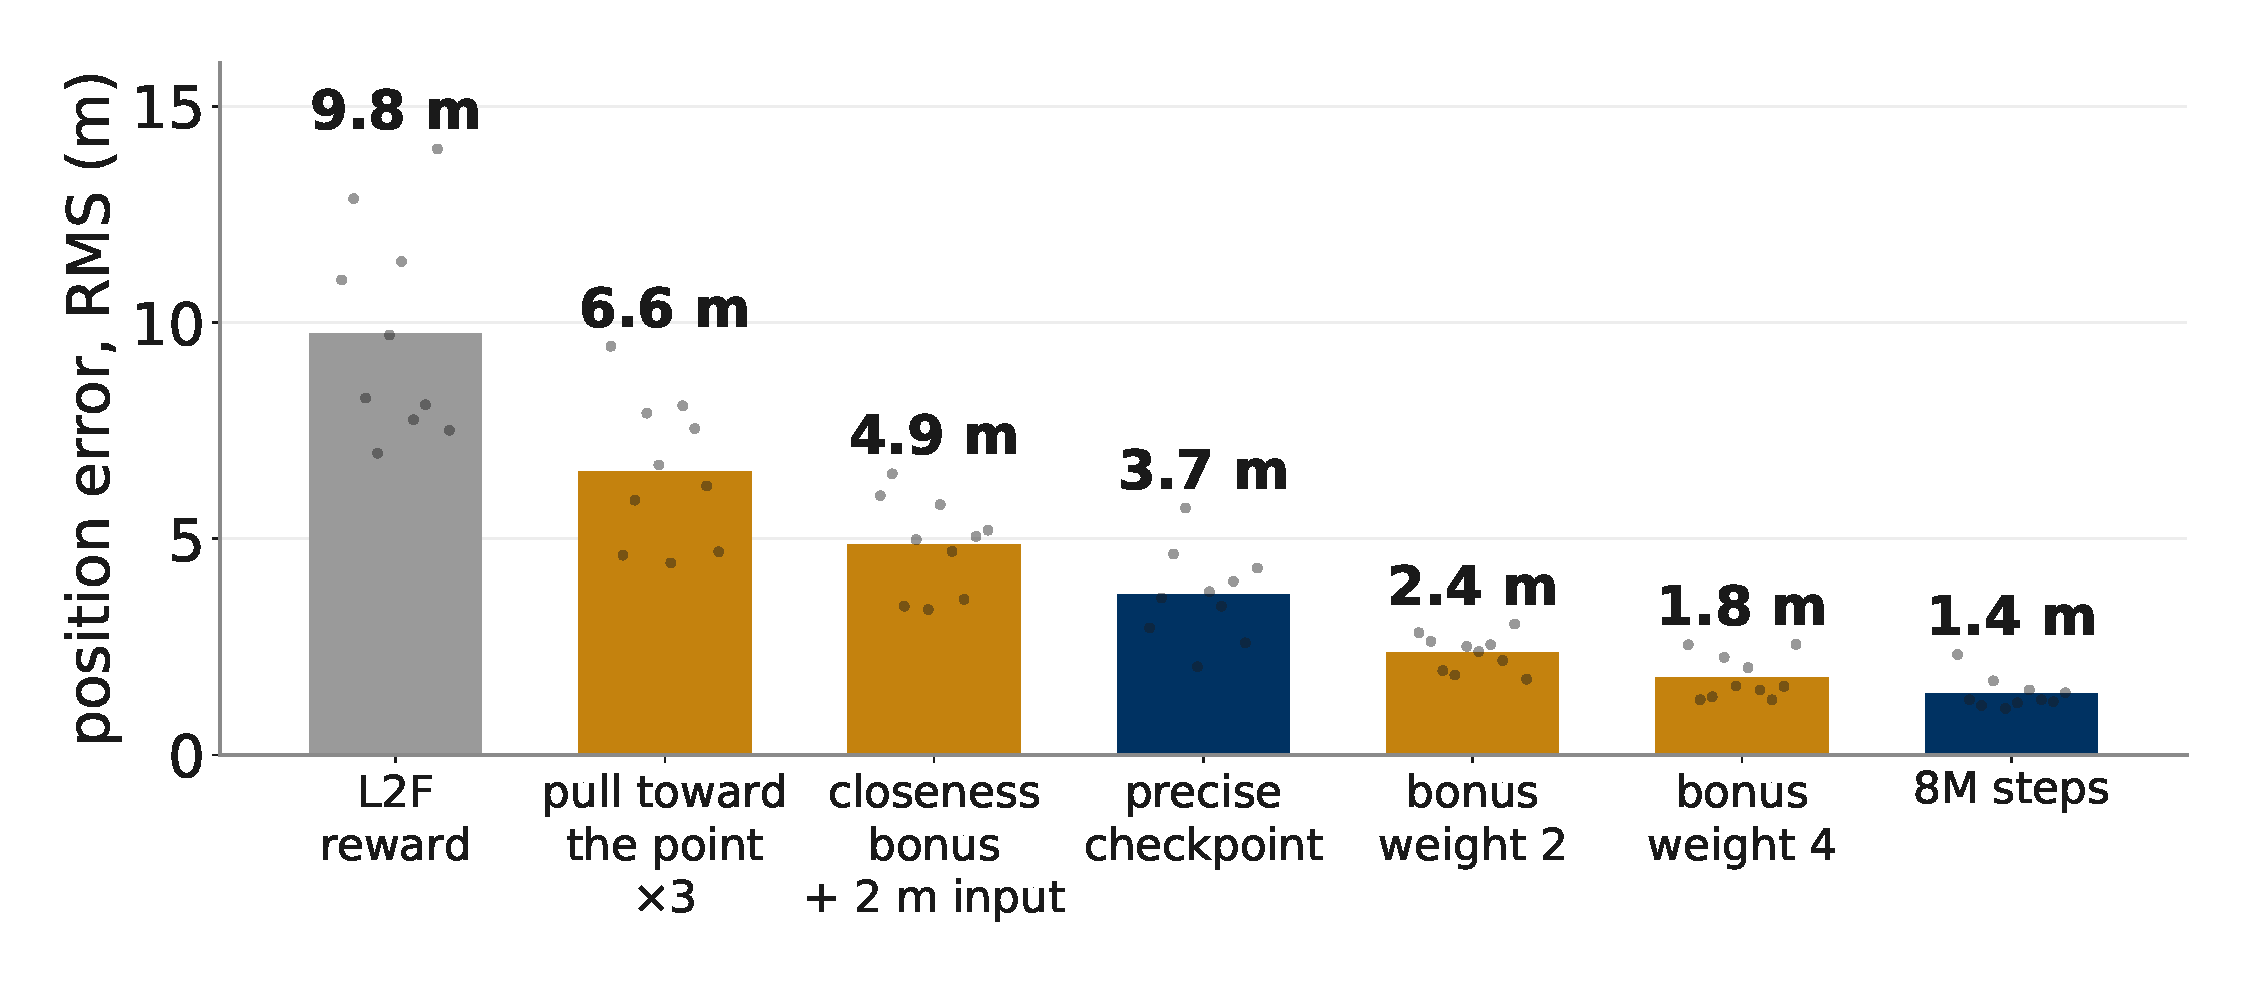
\includegraphics[width=16.8in]{figures/error.pdf}

{\note Test error over 10 training seeds (dots), best checkpoint, point flying straight; each bar keeps the changes on
its left. Gold: changes of the reward (the third bar also adds the 2~m input).}

\vspace{0.5em}
{\fontsize{32}{42}\selectfont
\[ r = 2 - \Big[\, w_p\Big(\frac{d}{20}\Big)^{2} + w_v\Big(\frac{\lVert v - v^{*}\rVert}{4}\Big)^{2}
      + w_\beta\Big(\frac{\beta}{5^\circ}\Big)^{2} + w_{\Delta a}\lVert\Delta a\rVert^{2} + w_\alpha m_\alpha^{2} \Big]
      \;{\color{gold}+\; w_b\, e^{-(d/\sigma)^{2}}} \]
\[ v^{*} = v_{\text{ref}} + {\color{gold}K}\,(p_{\text{ref}} - p) \]}

Squared costs are flat near the point: at the last stage, one meter of error costs 0.006 out of 2. Three changes
give the policy a reason to close the last meters: a stronger pull of the velocity target toward the point
({\color{gold}$K$}: 0.1 to 0.3~s$^{-1}$), a {\color{gold}bonus} that pays only near the point, its width $\sigma$
following half the mean training distance (weight 1, then 4), and the error also observed on a 2~m scale.

\vspace{0.4em}
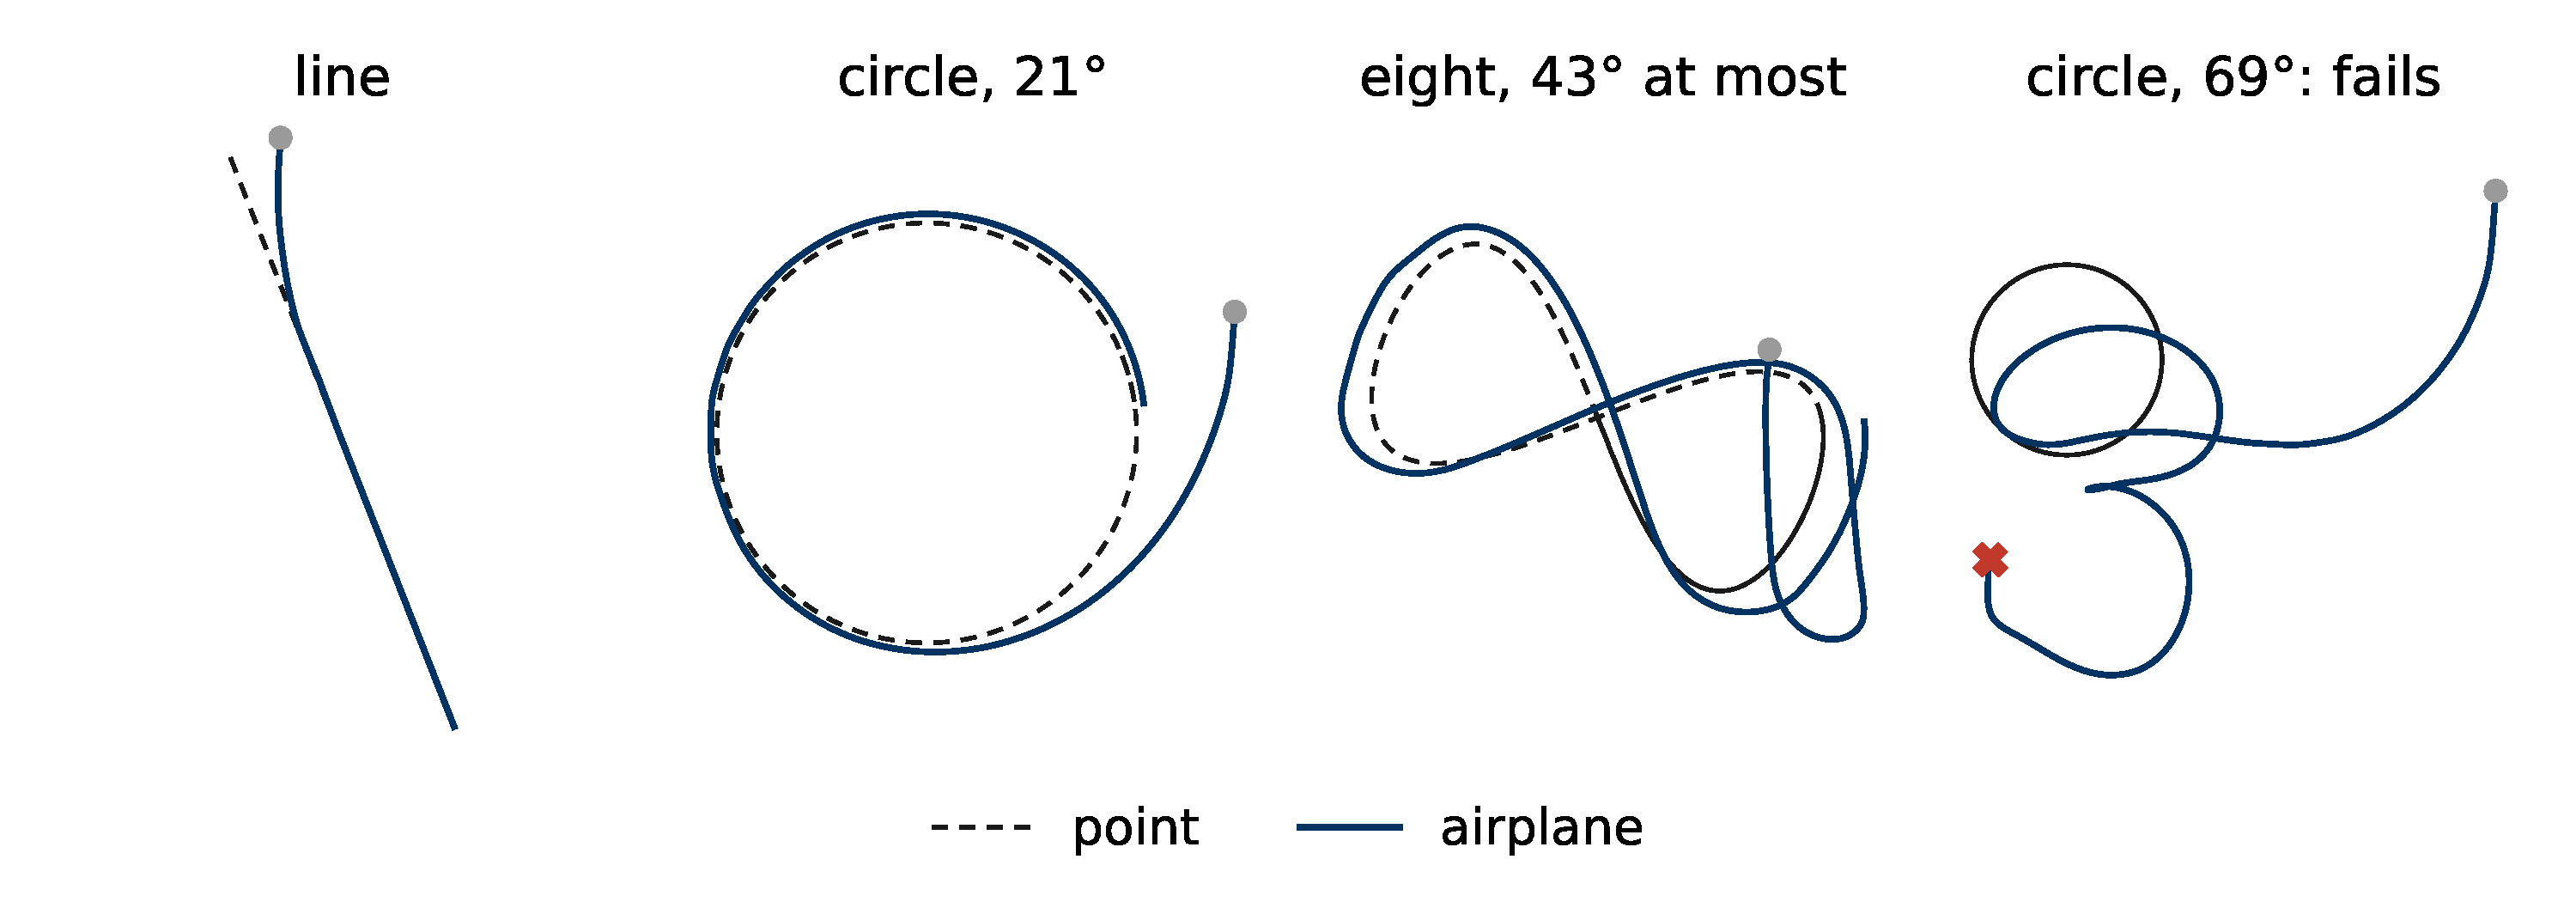
\includegraphics[width=16.8in]{figures/flights.pdf}

{\note Policy at 1.8~m (4M steps), one test flight per path (dashed: the point, grey dot: the airplane's start). Trained only on
straight lines.}

\vspace{0.6em}
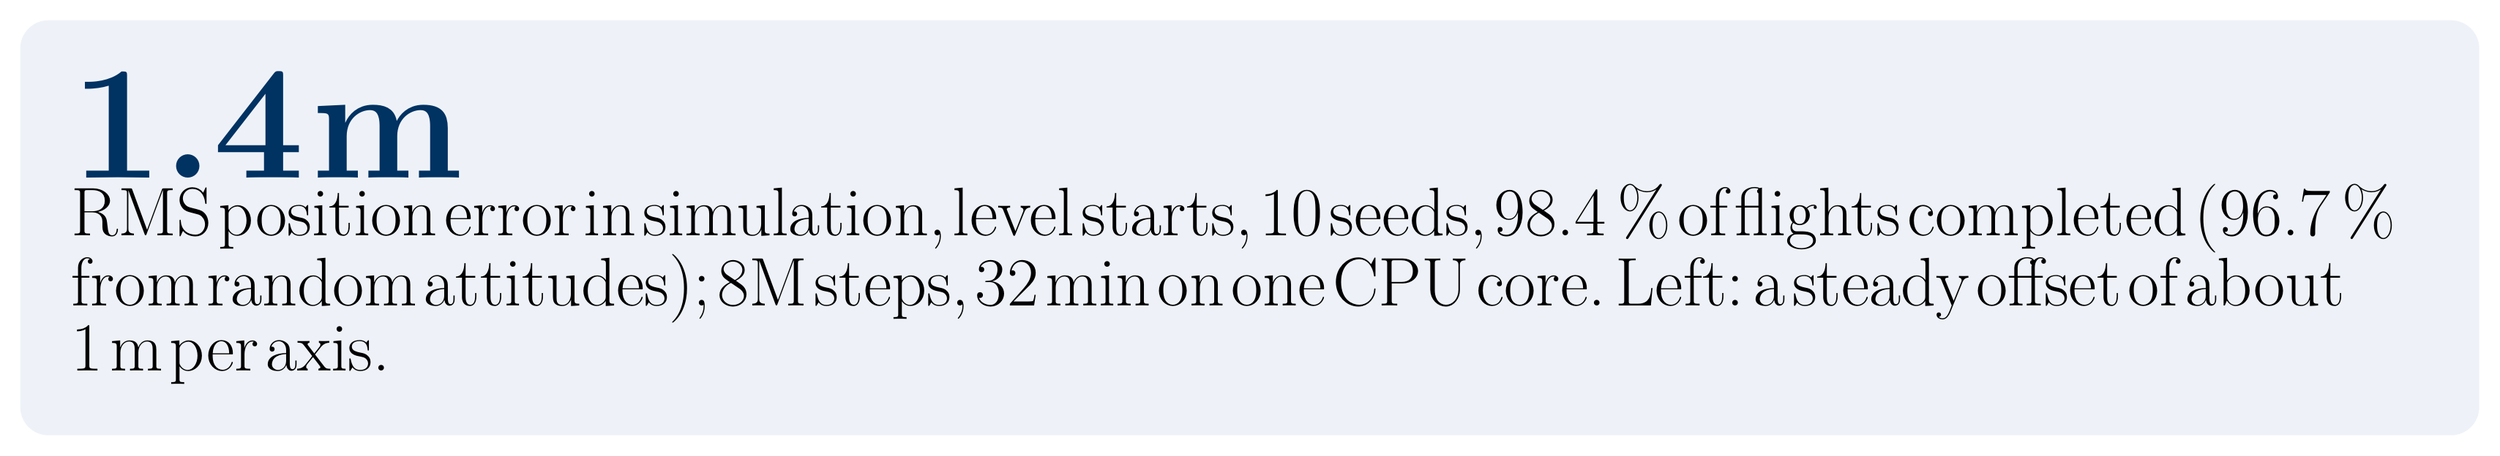
\begin{tikzpicture}[x=1in,y=1in]
  \node[fill=tint,rounded corners=14pt,inner sep=0.35in,text width=16.1in,align=left] {%
    \stat{1.4 m}{RMS position error in simulation, level starts, 10 seeds, 98.4\,\% of flights completed (96.7\,\%
    from random attitudes); 8M steps, 32~min on one CPU core. Left: a steady offset of about 1~m per axis.}};
\end{tikzpicture}
\end{minipage}%
\hspace{1.0in}%
% ----- column 3 -----------------------------------------------------------------------------------------------------
\begin{minipage}[t]{13.2in}
\body
\heading{Limit: points that turn}
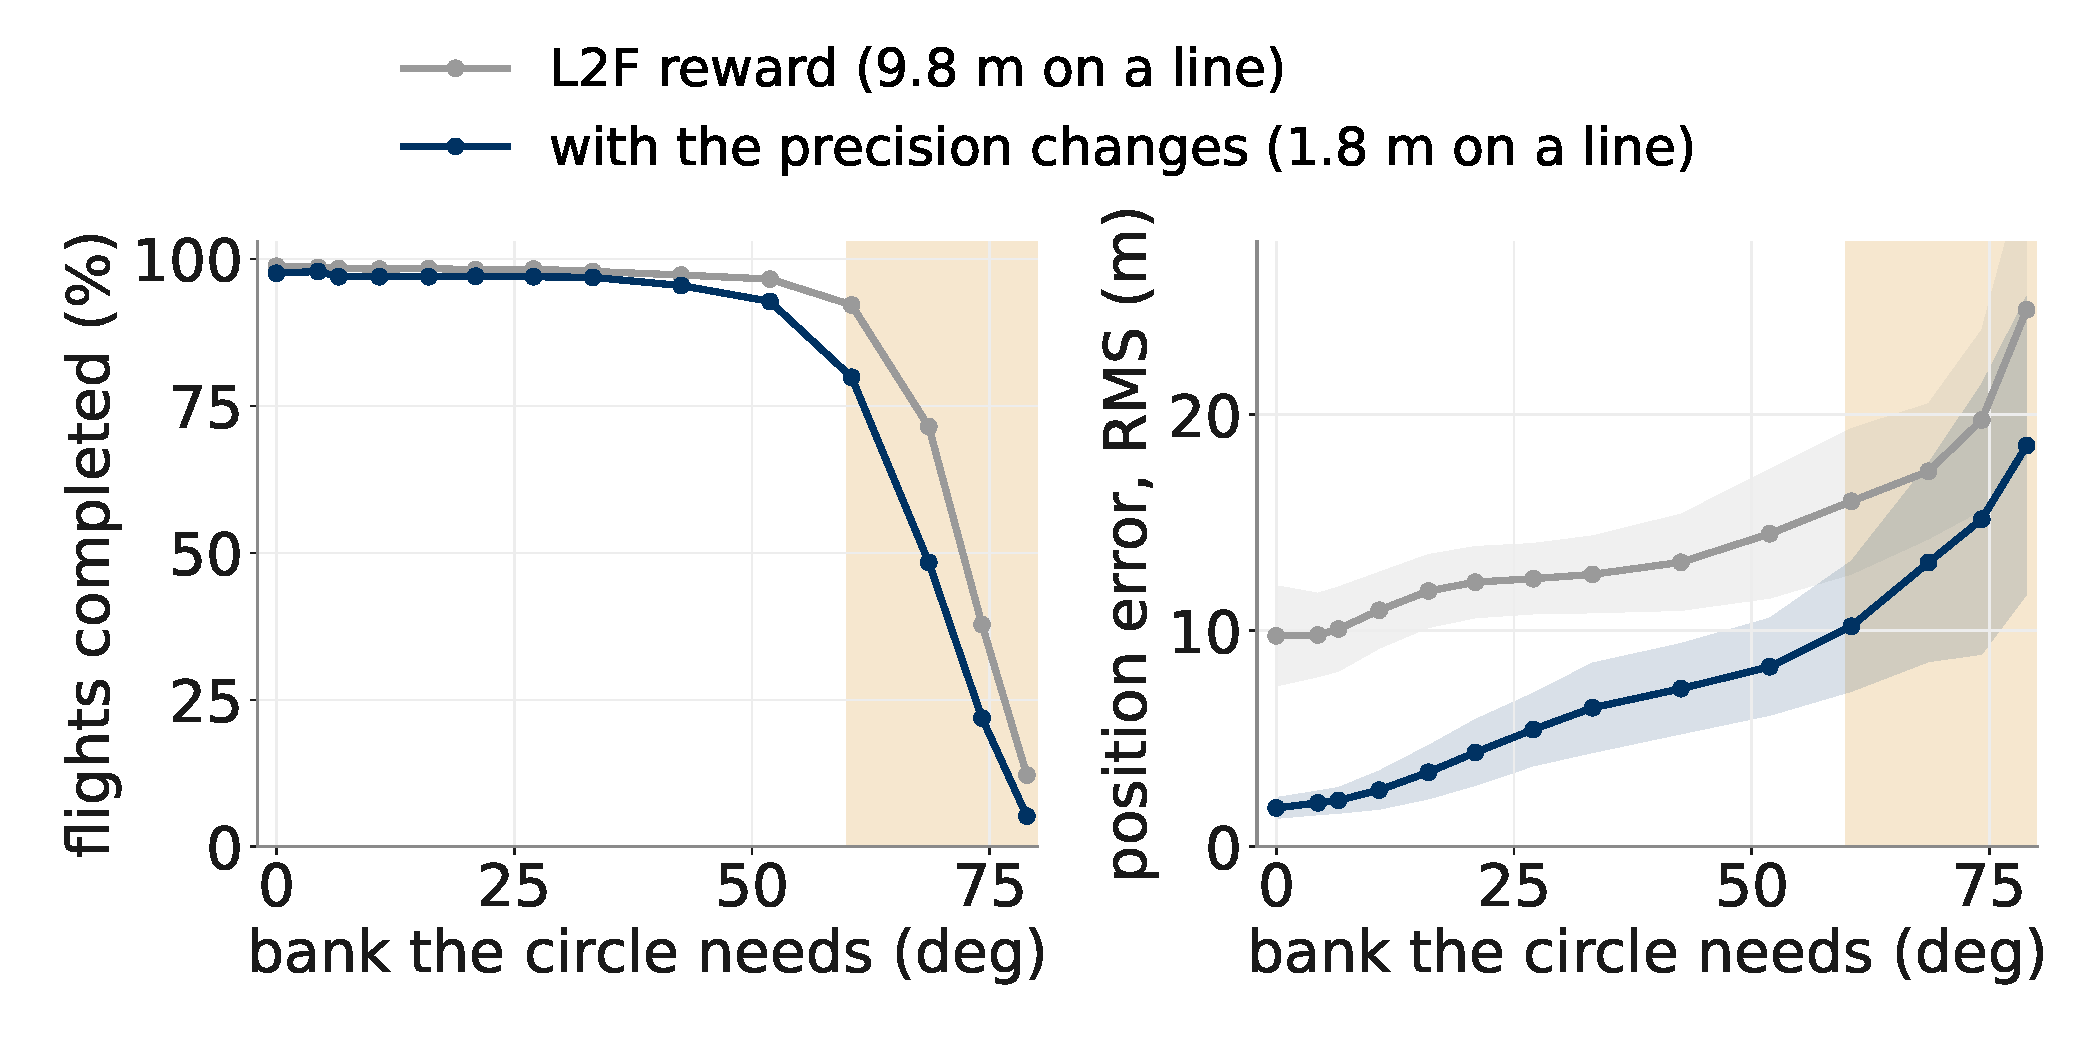
\includegraphics[width=13.2in]{figures/turning.pdf}

Up to 43$^\circ$ of bank the gain holds (7.3~m instead of 13.2~m), but the error grows as a lag; past
60$^\circ$ (shaded) the precise policies fail earlier. Next: train on turning points.

\heading{Training time}
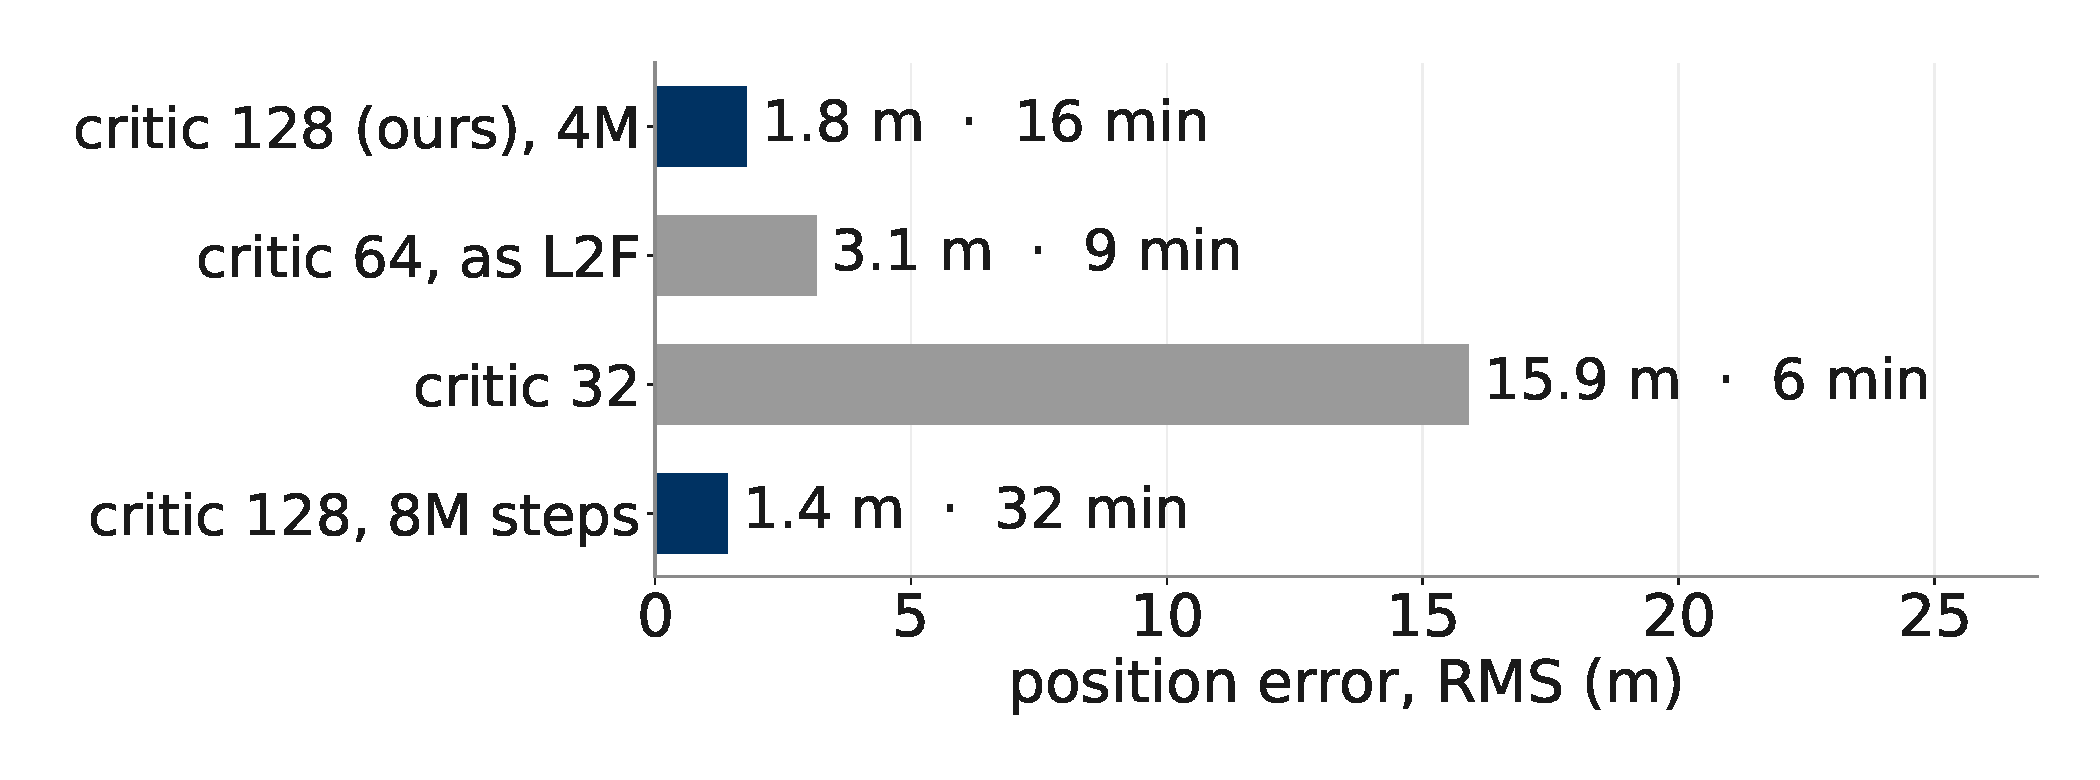
\includegraphics[width=13.2in]{figures/compute.pdf}

95\,\% of a training step is the network updates. Smaller critics lose the precision; more steps gain it.

\heading{Step 2: the lab's E-flite Eratix}
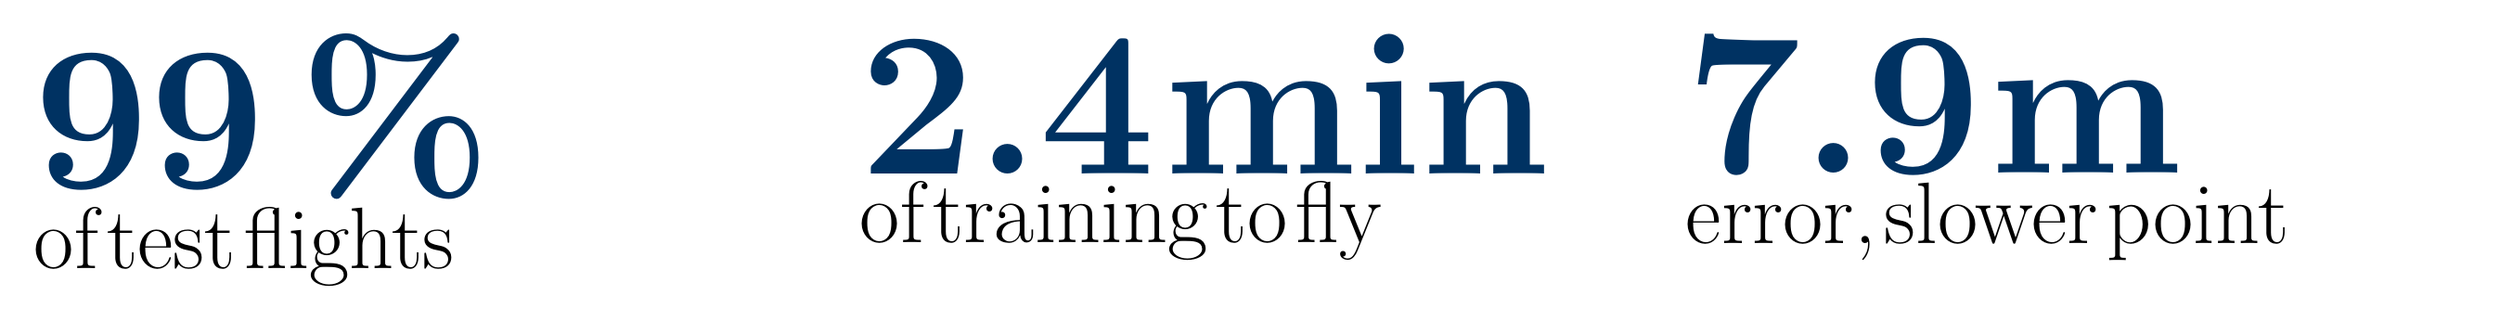
\begin{tikzpicture}[x=1in,y=1in]
  \node[anchor=north west,text width=4.0in] at (0,0) {\stat{99\,\%}{of test flights}};
  \node[anchor=north west,text width=4.0in] at (4.45,0) {\stat{2.4 min}{of training to fly}};
  \node[anchor=north west,text width=4.2in] at (8.9,0) {\stat{7.9 m}{error, slower point}};
\end{tikzpicture}

83~g, modelled from its specs; point at 7--10~m/s, earlier reward. Next: the changes of step 1.

\heading{Step 3: the real airplane}
Identify it from a few minutes of flight~[2], retrain with wind, noise and randomized parameters, fly it
through PX4. Not done yet.

\vspace{0.6em}
{\fontsize{25}{32}\selectfont\color{muted}
{[1]} J. Eschmann, D. Albani, G. Loianno, \emph{Learning to Fly in Seconds}, IEEE RA-L, 2024.\par
{[2]} J. Eschmann, D. Albani, G. Loianno, \emph{Data-Driven System Identification of Quadrotors Subject to Motor
Delays}, IROS, 2024.\par
{[3]} J. Eschmann, D. Albani, G. Loianno, \emph{RLtools: A Fast, Portable Deep Reinforcement Learning Library for
Continuous Control}, JMLR, 2024.\par
Code and results: github.com/clementdumeril/Fixed-Wing}
\end{minipage}
\end{document}
